\section{Eksperymenty numeryczne}
\label{eksperymenty_numeryczne}

Przeprowadzono szereg eksperymentów numerycznych. W każdym z nich badano jak zależy wyznaczone sterowanie optymalne od warunków początkowych i przyjętych ograniczeń (maksymalne napięcie lub maksymalne wychylenie). Oprócz tego badano również problem sterowania Segwayem dla różnych jego parametrów (np. zmieniając jego moment bezwładności). Dla każdego przeprowadzono eksperymentu zapisywano wygenerowane wykresy, a następnie je ze sobą porównywano.
\paragraph*{}
Pierwszy przeprowadzony eksperyment dotyczył problemu stabilizacji pozycji obiektu. W tym wypadku obiekt początkowo ustawiony był w niestabilnym punkcie równowagi:
\begin{equation}
x_0=\begin{bmatrix}
0\\
0\\
0\\
0\\
0
\end{bmatrix}
\end{equation}
Dla tego eksperymentu przyjęto następujące ograniczenia wychylenia, napięcia, współczynnik funkcji kary, liczbę węzłów strukturalnych oraz horyzont czasowy:
\begin{equation}
\begin{aligned}
\phi_{max}&=\frac{\pi}{18}\\
u_{max}&=8
K&=20\\
N&=16\\
T_{sim}&=2
\end{aligned}
\end{equation}

\begin{figure}[H]
	\centering
	\subfloat{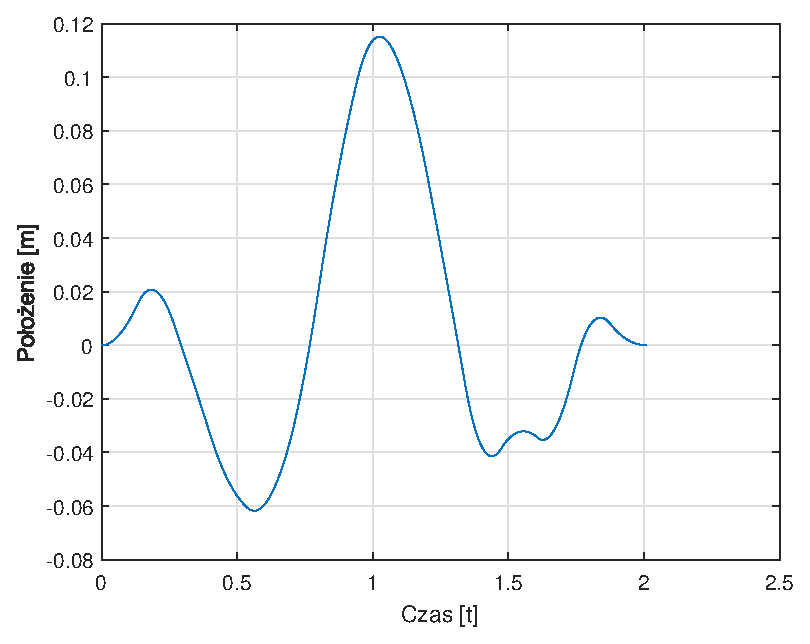
\includegraphics[width=2.8in]{Figures/equ_pos.eps}}
	~~
	\subfloat{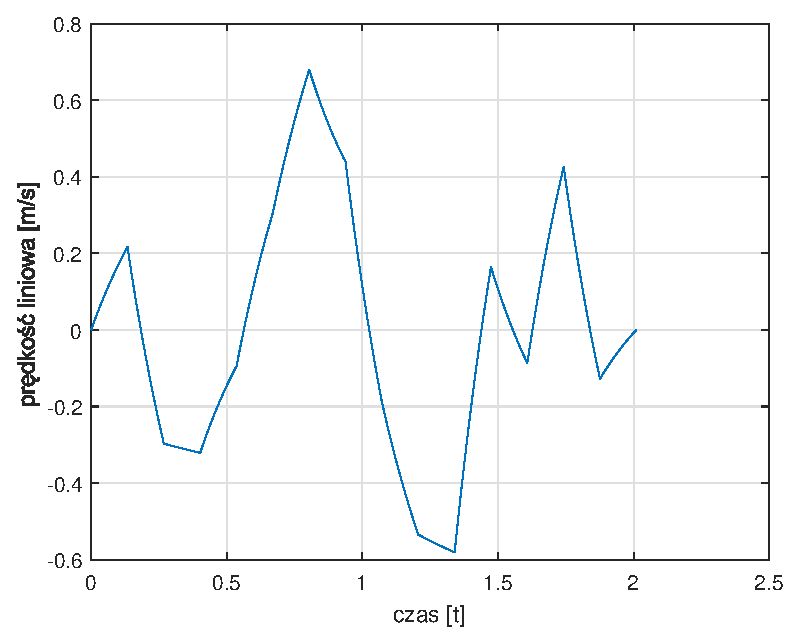
\includegraphics[width=2.8in]{Figures/equ_vel.eps}}
	
	\subfloat{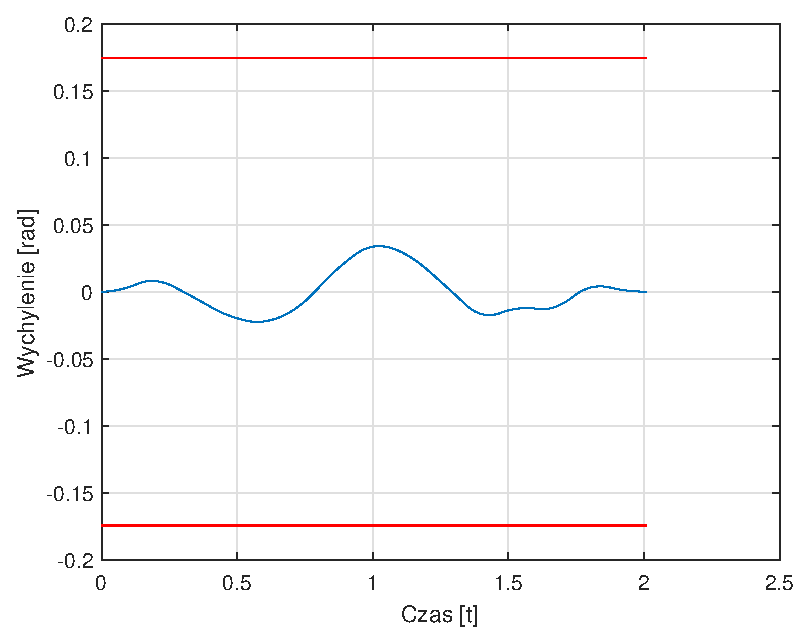
\includegraphics[width=2.8in]{Figures/equ_ang.eps}}
	~~
	\subfloat{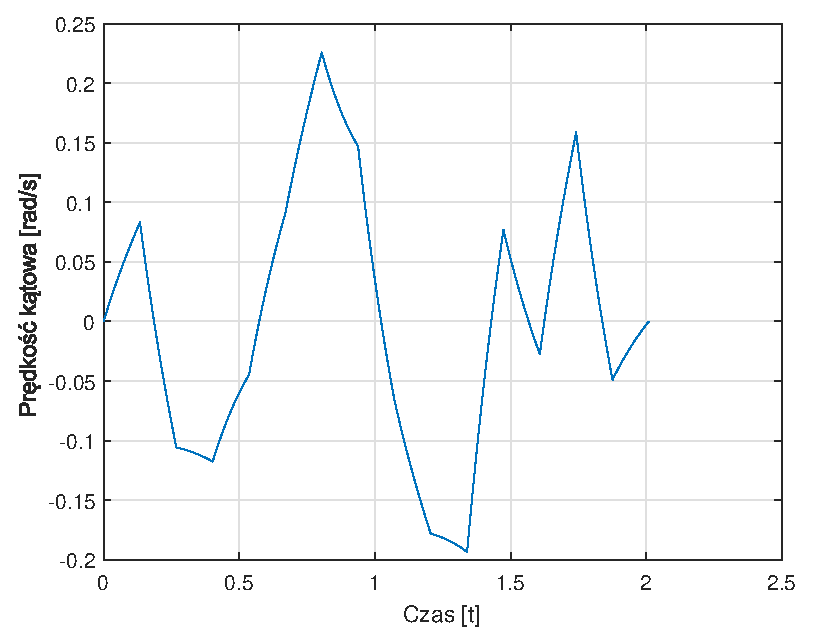
\includegraphics[width=2.8in]{Figures/equ_ang_vel.eps}}
	
	\subfloat{\includegraphics[width=2.8in]{Figures/equ_pen.eps}}
	~~
	\subfloat{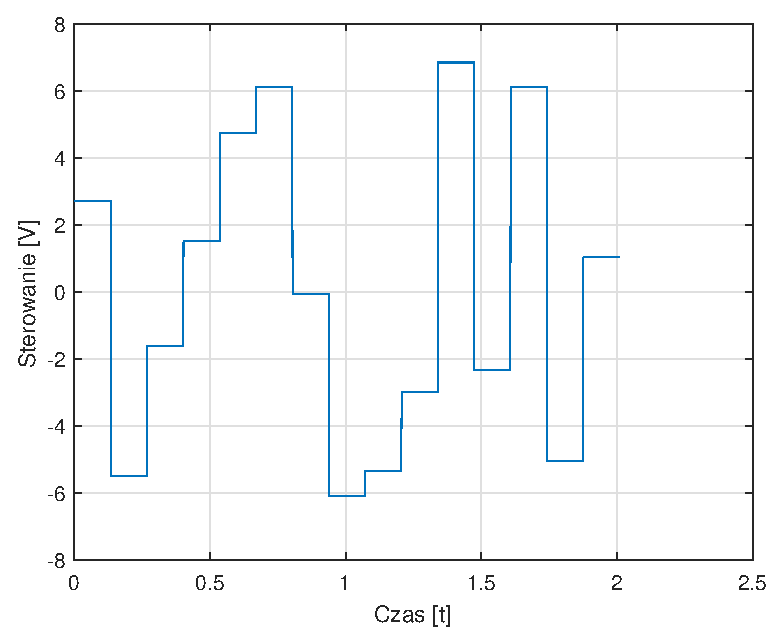
\includegraphics[width=2.8in]{Figures/equ_con.eps}}
	\caption{Zadanie stabilizacji obiektu w punkcie równowagi.}
	\label{fig:equ}
\end{figure}

Koszt dla sterowania pokazanego na rysunku \ref{fig:stab} wynosi około \(5.69 \cdot 10^{-16}\). Obiekt pod koniec symulacji znajdował się bardzo blisko zadanej pozycji. Dziwić może fakt, że obiekt został wytrącony z położenia równowagi, mimo, że znajdował się w nim już na początku symulacji.

\newpage
Następnym eksperymentem było zbadanie stabilizacji układu, gdy warunek początkowy nie znajduje się w punkcie równowagi. Wybrano następujący warunek początkowy:
\begin{equation}
x_0=\begin{bmatrix}
-2\\
0\\
0\\
0\\
0
\end{bmatrix}
\end{equation}
Dla tego eksperymentu przyjęto następujące ograniczenia wychylenia, napięcia, współczynnik funkcji kary, liczbę węzłów strukturalnych oraz horyzont czasowy:
\begin{equation}
\begin{aligned}
\phi_{max}&=\frac{\pi}{18}\\
u_{max}&=13
K&=30\\
N&=16\\
T_{sim}&=2.5
\end{aligned}
\end{equation}

\begin{figure}[H]
	\centering
	\subfloat{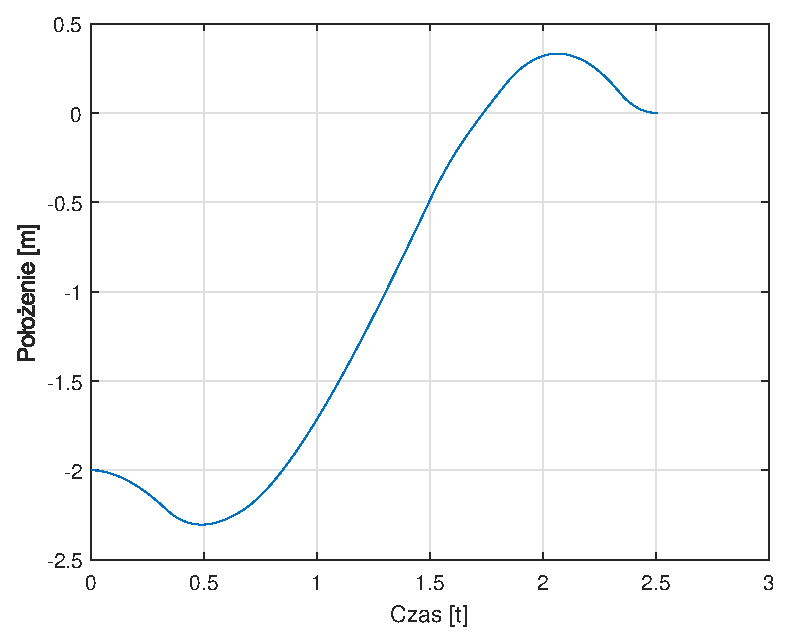
\includegraphics[width=2.8in]{Figures/stab_pos.eps}}
	~~
	\subfloat{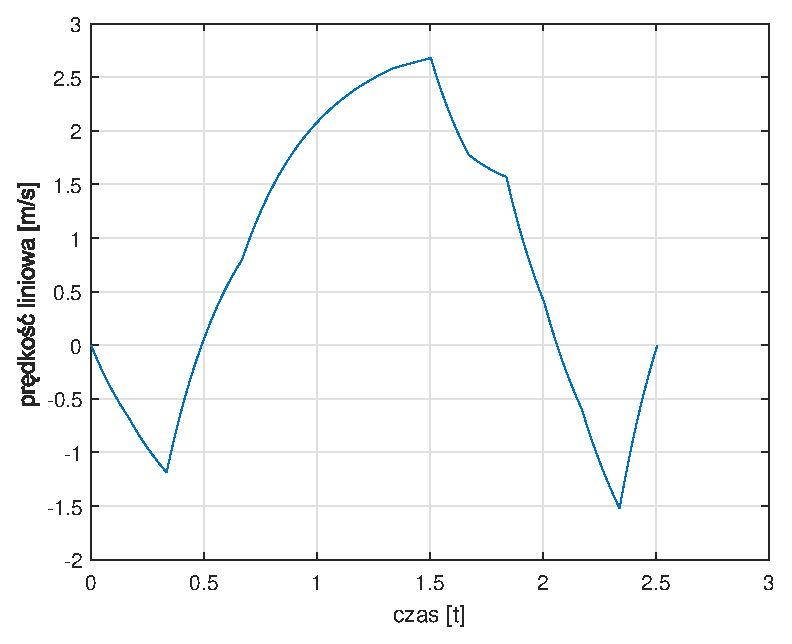
\includegraphics[width=2.8in]{Figures/stab_vel.eps}}
	
	\subfloat{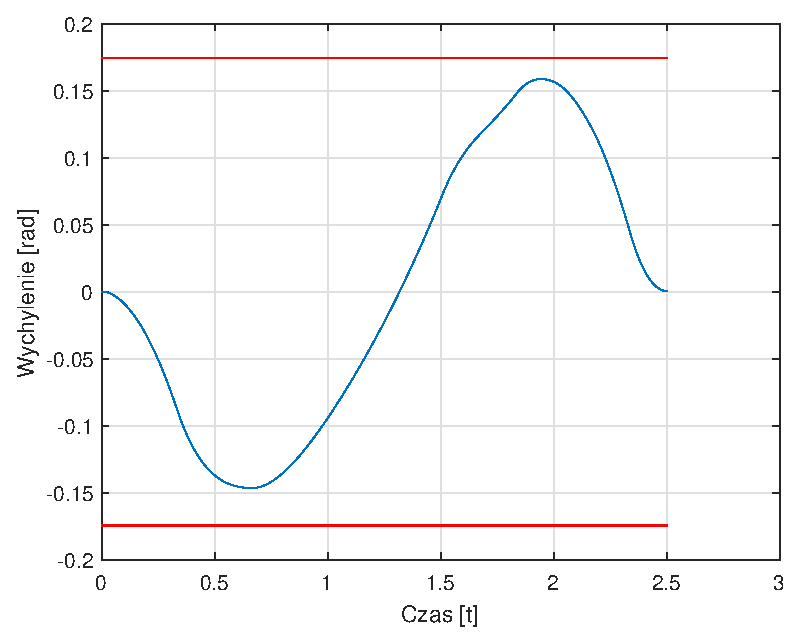
\includegraphics[width=2.8in]{Figures/stab_ang.eps}}
	~~
	\subfloat{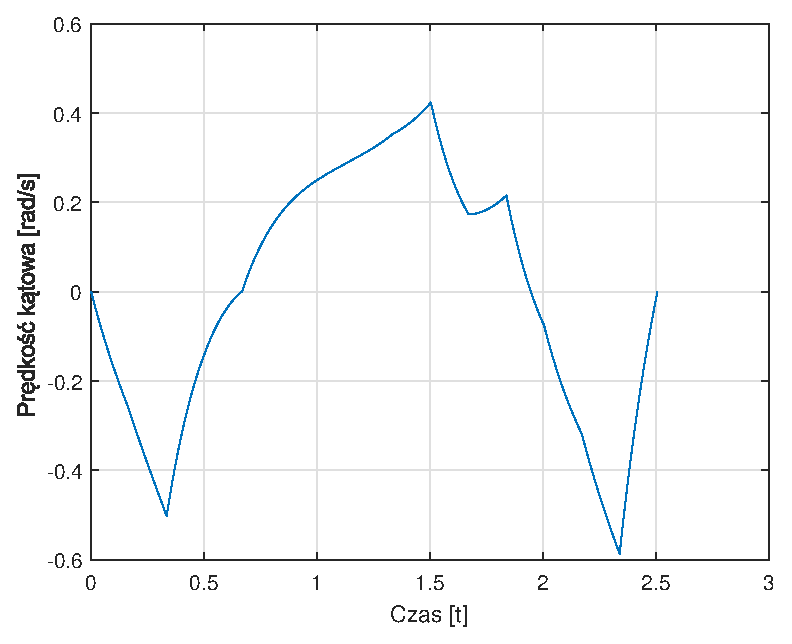
\includegraphics[width=2.8in]{Figures/stab_ang_vel.eps}}
	
	\subfloat{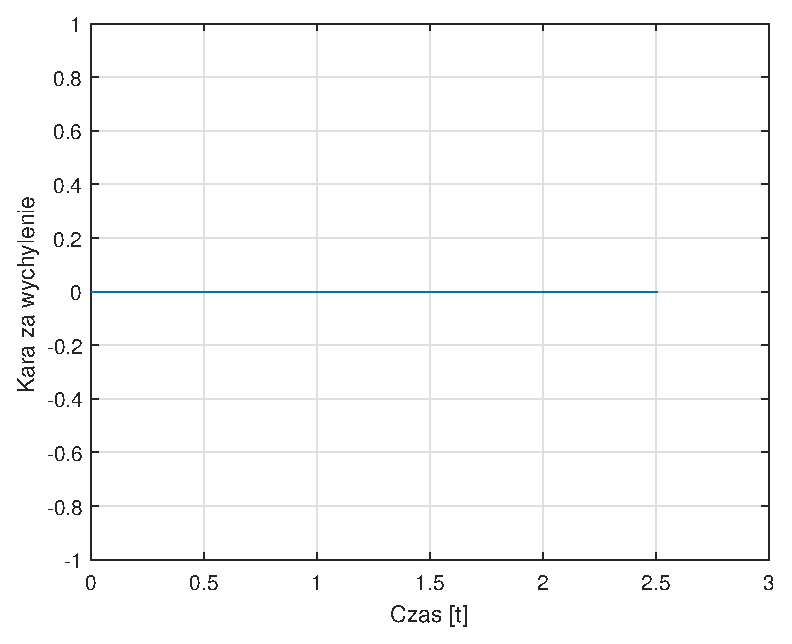
\includegraphics[width=2.8in]{Figures/stab_pen.eps}}
	~~
	\subfloat{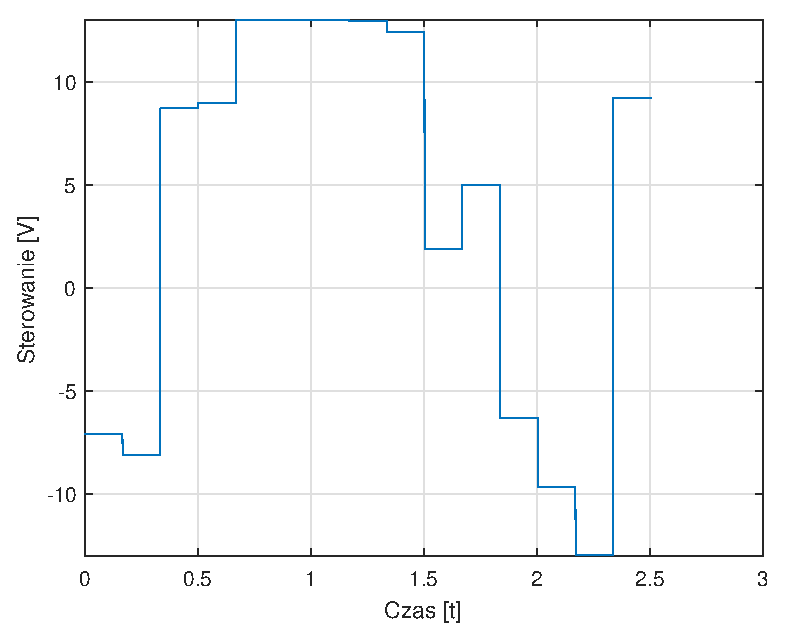
\includegraphics[width=2.8in]{Figures/stab_con.eps}}
	\caption{Zadanie stabilizacji obiektu w punkcie równowagi dla innych warunków początkowych.}
	\label{fig:stab}
\end{figure}

Koszt dla sterowania pokazanego na rysunku \ref{fig:stab} wynosi około \(1.72 \cdot 10^{-17}\). Świadczy to o tym, że obiekt jest pozycjonowanie bardzo dokładnie, a odchylenia od pozycji zadanej po upływie czasu symulacji są praktycznie zerowe.

\newpage
W kolejnym podejściu przetestowano zdolność systemu do pokonywania określonego dystansu z zachowaniem warunku co do maksymalnego wychylenia. Wybrano następujący warunek początkowy:
\begin{equation}
x_0=\begin{bmatrix}
-1\\
0\\
0\\
0\\
0
\end{bmatrix}
\end{equation}
Przyjęto parametry:
\begin{equation}
\begin{aligned}
\phi_{max}&=\frac{\pi}{18}\\
u_{max}&=20\\
K&=300\\
N&=10
\end{aligned}
\end{equation}
gdzie \textit{K} jest współczynnikiem kary za nadmierne wychylenie, natomiast \textit{N} oznacza liczę węzłów strukturalnych.\\
Badano zachowania systemu dla różnych chwil końcowych. Najbardziej zadowalające wyniki otrzymana dla czasu $\textit{T}=1.6 s$ (\ref{fig:equ1}). Wskaźnik jakości osiągnął wartość\\ $Q(u^*)=3.31\cdot10^{-4}$.
\begin{figure}[H]
	\centering
	\subfloat{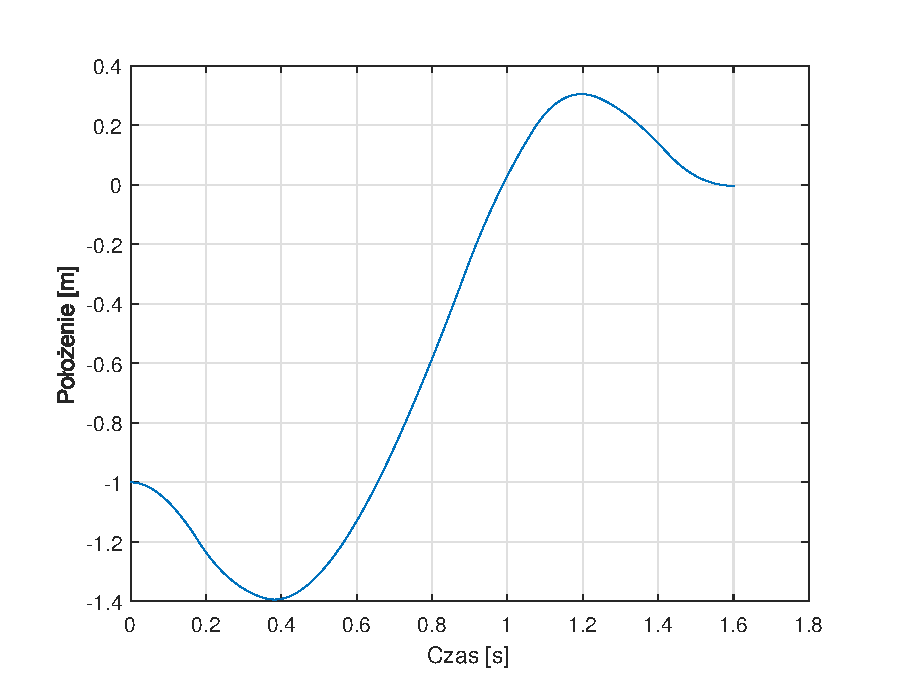
\includegraphics[width=2.8in]{Figures/exp1/pos.eps}}
	~~
	\subfloat{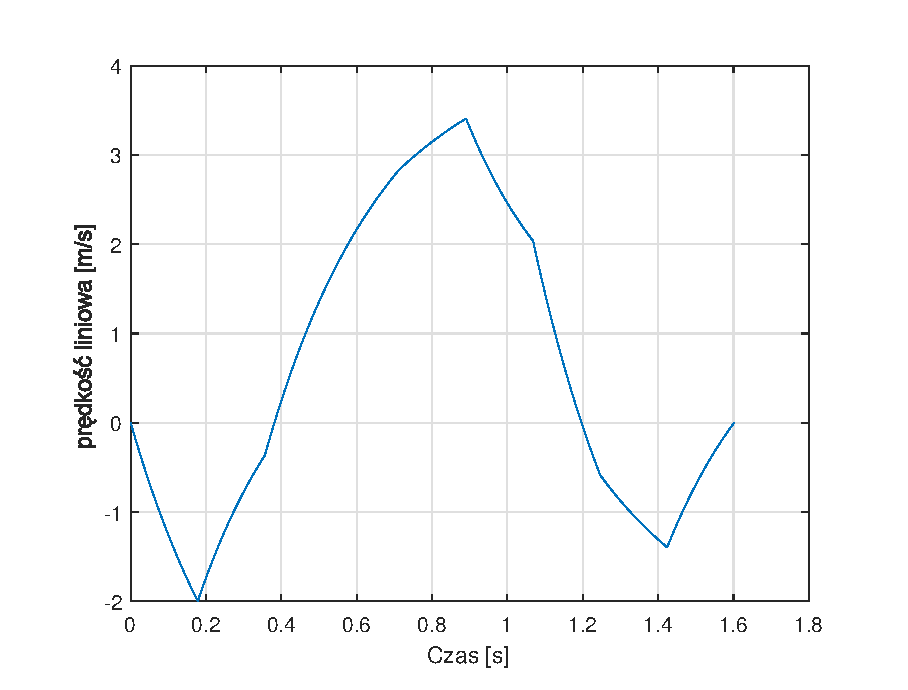
\includegraphics[width=2.8in]{Figures/exp1/vel.eps}}
	
	\subfloat{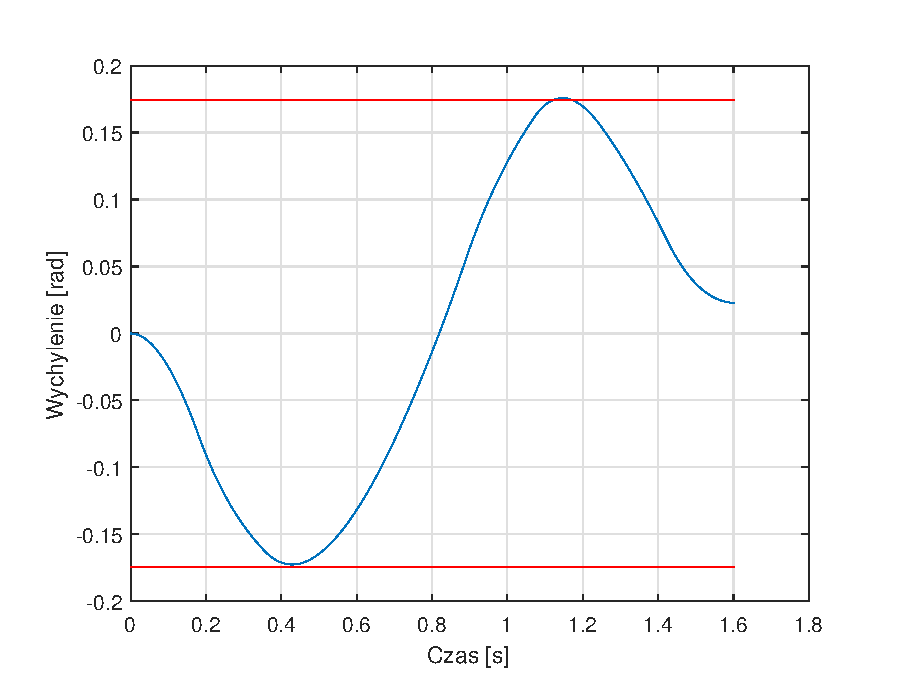
\includegraphics[width=2.8in]{Figures/exp1/ang.eps}}
	~~
	\subfloat{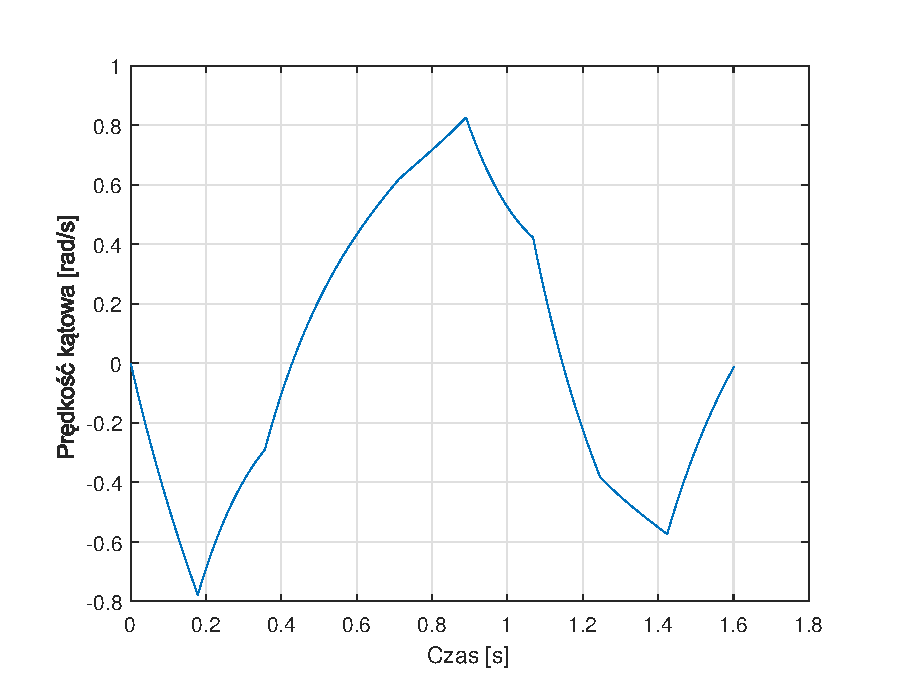
\includegraphics[width=2.8in]{Figures/exp1/ang_vel.eps}}
	
	\subfloat{\includegraphics[width=2.8in]{Figures/exp1/pen.eps}}
	~~
	\subfloat{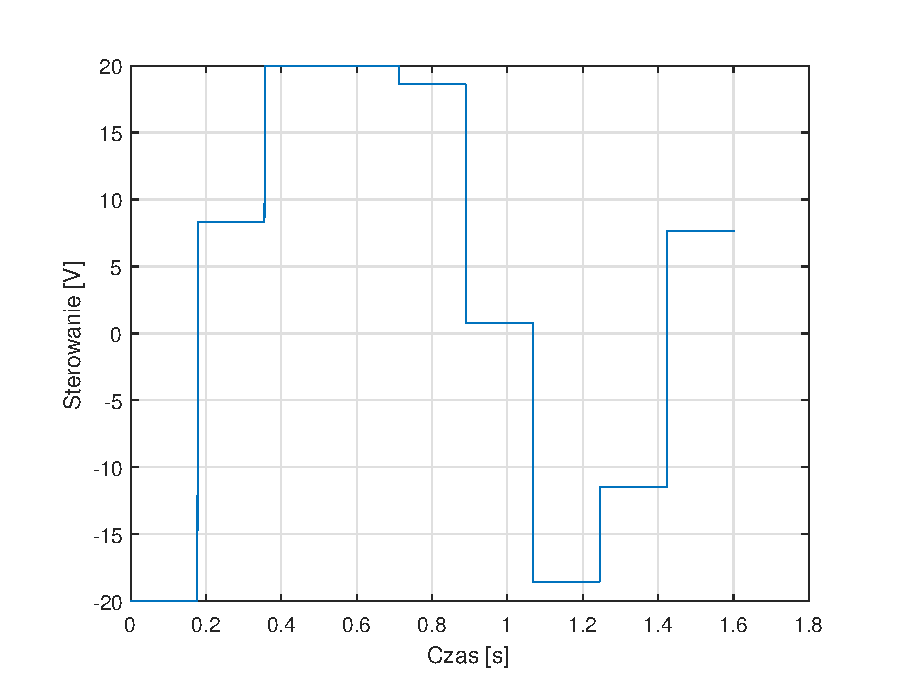
\includegraphics[width=2.8in]{Figures/exp1/control.eps}}
	\caption{Seqway pokonuje dystans 1 metra w czasie 1.6 sekundy.}
	\label{fig:equ1}
\end{figure}
Przyjmując za rozwiązanie początkowe $u^*$ oraz zwiększając współczynnik kary $K=3\cdot10^6$ przeprowadzono kolejną symulację. Zauważono, że postać rozwiązanie nie zmieniła się znacząco. Kara za wychylenie zmalała o trzy rzędy, a nowy wskaźnik jakości wyniósł    $Q(u_2^*)=2.01\cdot10^{-4}$. W obu przypadkach zdecydowanie największy wpływ na wskaźnik jakości miało niezerowe wychylenie w chwili końcowej. Dostrzegając różnicę pomiędzy wskaźnikami jakości postanowiono podążyć dalej podobnym tokiem rozumowania. Po kilkukrotnym wywołaniu programu optymalizującego z nowo wyliczonymi rozwiązaniami otrzymano następującą postać sterowania (\ref{fig:ctrNew}):
\begin{figure}[H]
	\centering
	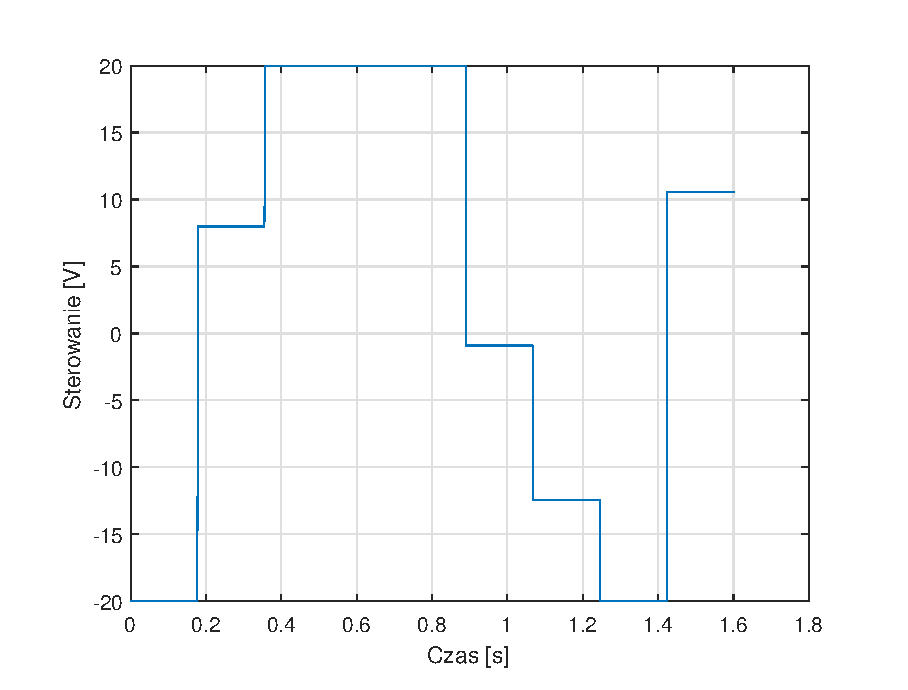
\includegraphics[width=4in]{Figures/exp1/controlNew.eps}
	\caption{Sterowanie otrzymane w wyniku kilkukrotnej optymalizacji.}
	\label{fig:ctrNew}
\end{figure}
Sterowanie wyraźnie bardziej opiera się na ograniczeniach. Finalna wartość wskaźnika jakości wyniosła $Q(u_f^*)=1.64\cdot10^{-4}$.